\documentclass{sig-alternate}
\usepackage{enumitem}
\usepackage{multirow}
\usepackage{amsmath}
\usepackage{amssymb}
\usepackage{adjustbox}

\begin{document}

% Copyright
\setcopyright{acmcopyright}
%\setcopyright{acmlicensed}
%\setcopyright{rightsretained}
%\setcopyright{usgov}
%\setcopyright{usgovmixed}
%\setcopyright{cagov}
%\setcopyright{cagovmixed}


% DOI
\doi{10.475/123_4}

% ISBN
\isbn{123-4567-24-567/08/06}

%Conference
\conferenceinfo{DLfM '16}{June 12, 2016, New York, NY, USA}

\acmPrice{\$15.00}

%
% --- Author Metadata here ---
\conferenceinfo{3rd International Digital Libraries for Musicology workshop (DLfM)}{2016 New York, USA}
%\CopyrightYear{2007} % Allows default copyright year (20XX) to be over-ridden - IF NEED BE.
%\crdata{0-12345-67-8/90/01}  % Allows default copyright data (0-89791-88-6/97/05) to be over-ridden - IF NEED BE.
% --- End of Author Metadata ---

\title{MORTY: A Toolbox for \\Mode Recognition and Tonic Identification}

\numberofauthors{3}
\author{
% You can go ahead and credit any number of authors here,
% e.g. one 'row of three' or two rows (consisting of one row of three
% and a second row of one, two or three).
%
% The command \alignauthor (no curly braces needed) should
% precede each author name, affiliation/snail-mail address and
% e-mail address. Additionally, tag each line of
% affiliation/address with \affaddr, and tag the
% e-mail address with \email.
%
% 1st. author
\alignauthor
Altu\u{g} Karakurt\\
       \affaddr{Bilkent University}\\
       \affaddr{1932 Wallamaloo Lane}\\
       \affaddr{Wallamaloo, New Zealand}\\
       \email{trovato@corporation.com}
% 2nd. author
\alignauthor
Sertan \c{S}ent\"{u}rk, \\
       \affaddr{Universitat Pompeu Fabra}\\
       \affaddr{Roc Boronat, 138}\\
       \affaddr{Barcelona, Spain 08018}\\
       \email{sertan.senturk@upf.edu}
% 3rd. author
\alignauthor Xavier Serra\\
       \affaddr{Universitat Pompeu Fabra}\\
       \affaddr{Roc Boronat, 138}\\
       \affaddr{Barcelona, Spain 08018}\\
       \email{xavier.serra@upf.edu}
}
\date{submitted: 20 May 2016}

\maketitle
\begin{abstract}
In the general sense, mode defines the melodic framework and tonic acts as the reference tuning pitch for the melody in the performances of many music cultures. The mode and the tonic information of the audio recordings is essential for many music information retrieval tasks such as automatic transcription, tuning analysis and music similarity and automatic description of digital music libraries applied to these cultures. In this paper we present MORTY, an open source toolbox for mode recognition and tonic identification. The toolbox implements a generalized variant of two state-of-the-art methods based on pitch distribution analysis. The algorithms are designed in a generic manner such that they can be easily optimized according to the culture-specific aspects of the studied music tradition. We test the generalized methodology systematically on the largest mode recognition dataset curated for Ottoman-Turkish makam music so far, which is composed of 1000 recordings in 50 modes. We obtained 94.9\%, 71.4\% and 63.2\% accuracy in tonic identification, mode recognition and joint estimation of the mode and tonic tasks, respectively. We additionally present recent experiments on Carnatic and Hindustani music in comparison with several methodologies recently proposed for raga/raag recognition and our preliminary experiments for mode recognition using neural networks. We believe that our toolbox would be used as a benchmark for future methodologies proposed for mode recognition and tonic identification, especially for music traditions in which these computational tasks have not been addressed yet.

\end{abstract}

\begin{CCSXML}
<ccs2012>
 <concept>
  <concept_id>10010520.10010553.10010562</concept_id>
  <concept_desc>Computer systems organization~Embedded systems</concept_desc>
  <concept_significance>500</concept_significance>
 </concept>
 <concept>
  <concept_id>10010520.10010575.10010755</concept_id>
  <concept_desc>Computer systems organization~Redundancy</concept_desc>
  <concept_significance>300</concept_significance>
 </concept>
 <concept>
  <concept_id>10010520.10010553.10010554</concept_id>
  <concept_desc>Computer systems organization~Robotics</concept_desc>
  <concept_significance>100</concept_significance>
 </concept>
 <concept>
  <concept_id>10003033.10003083.10003095</concept_id>
  <concept_desc>Networks~Network reliability</concept_desc>
  <concept_significance>100</concept_significance>
 </concept>
</ccs2012>  
\end{CCSXML}

\ccsdesc[500]{Computer systems organization~Embedded systems}
\ccsdesc[300]{Computer systems organization~Redundancy}
\ccsdesc{Computer systems organization~Robotics}
\ccsdesc[100]{Networks~Network reliability}

\printccsdesc

\keywords{Mode recognition; Tonic Identification; Toolbox; Ottoman-Turkish makam music; Carnatic Music; Hindustani Music; Pitch Class Distribution; $k$-nearest neighbors classification}

\section{Introduction}\label{sec:introduction}
In many music cultures, the mode specifies the scale and melodic characteristics of the music. Mode recognition is an important task for computational musicology to study the underlying phenomena behind this concept. Tonic is the reference frequency of a recording, which is used to determine the frequencies that correspond to the notes of the studied musical tradition. Many modal music cultures don't have a consensus on frequency values for notes, which makes it crucial to identify the tonic frequency correctly. Knowing it allows us to reveal the mapping of notes to frequencies and to computationally study pitch-related properties of a recording. This mapping also makes it possible to compare such properties of multiple recordings independent from their potentially different tonic frequencies. Hence, estimating the tonic of a recording is the first step for various tasks, such as tuning analysis~\cite{tuning}, and automatic transcription~\cite{transcription}. One of our motivations for this work is to provide dependable tools to be used for such higher level tasks for modal music cultures.

We present MORTY, an open source toolbox for mode recognition and tonic identification. It contains three pitch histogram based methods, two of which are state of the art algorithms proposed for specific modal music traditions. We provide generalized implementations of these that can be used for any modal music culture, as well as our multi-layer perceptron neural network specialized for mode recognition. Our neural network implementation uses the pitch histogram of recordings to recognize their modes.

We consider unavailability of public tools and datasets, as well as lack of reproduciblity to be some of the biggest obstacles in front of the progress of not only computational musicology, but for computational research in general. Our aim is to propose our primary work on applying neural networks on modal music information retrieval and to pave the way for future research on modal music, by providing the open source implementations of state of the art algorithms and our approach together with a public dataset for evaluation. Accessibility of such tools and data would help the researchers quantify the performances of their novel algorithms and compare them with the state-of-the-art.

Our contributions can be summarized as:
\begin{enumerate}[noitemsep]
\item An open toolbox aimed to set a benchmark for future research in mode recognition and tonic identification, which implements and generalizes the state of the art methodologies propo\-sed by Bozkurt and Ge\-dik~\cite{bozkurt_tonic, bozkurt_makam}, and Chordia and \c{S}ent\"{u}rk~\cite{chordia}
\item The largest makam recognition dataset for Ottoman-Turkish Makam Music (OTMM), composed of 1000 audio recordings from 20 makams with annotated tonic frequency and editorial metadata.
\item Exhaustive and reproducible evaluation of the aforementioned two state of the art methods on the Otto\-man-Turkish makam recognition dataset.
\item Improvements in the state of the art for tonic identification in OTMM
\item The first neural network based algorithm for culture-independent mode recognition and its open source implementation. 
\item Experiments on Hindustani and Carnatic music traditions to demonstrate the applicability of the implementations on different music cultures.
\end{enumerate}
The rest of this paper is organized as the following: In Section~\ref{sec:music} we provide the musical background relevant to these problems and methods. Section~\ref{sec:problem} provides a formal definition of the problem. Section~\ref{sec:stateoftheart} presents the current state-of-the-art. Section~\ref{sec:methodology} describes the methods and their implementations in detail. Section~\ref{sec:dataset} introduces the Ottoman-Turkish makam recognition dataset. Section~\ref{sec:experiments} explains the experiments and the obtained results. Finally, we discuss the results we obtained in Section~\ref{sec:discussion} and conclude with our comments and suggestions for the future work in Section~\ref{sec:conclusion}.


\section{Musical background}\label{sec:music}

define mode in "broad sense"? mode and tonic have synonymous meanings in many music cultures. tonal does not explain this concept. nasil cesitlidir? ornekler: makam, raag, raga, church modes etc. we should introduce what a stable pitch is. should we explain mono-/poly-/hetero-phony?

tonic as the reference for melody.

\section{Problem Definition}\label{sec:problem}
We define \emph{mode recognition} as classifying the mode $\zeta^{(a)}$ of an audio recording $(a)$ from a discrete set of modes $Z = \{\zeta_1, \dots, \zeta_V\}$, where $\zeta^{(a)} \in Z$ and $V$ is the total number of modes. The mode set is specific to music culture being studied. In mode recognition, we assume that the tonic frequency $r^{(a)}$ of the audio recording is available.

We define \emph{tonic identification} as estimating the frequency or the pitch class (if the octave information of the tonic is not be well-defined\footnote{e.g. orchestral recordings of OTMM as explained in Section~\ref{sec:experiments}}), $r^{(a)}$ of the performance tonic. Unlike modes, frequency is a continuous variable. However, in practice, the tonic is typically constrained to be one of the stable pitches performed~\cite{chordia,bozkurt_makam}. With this assumption, tonic identification can be reformulated as estimating the tonic frequency or the pitch class $r^{(a)}$ from a finite set of stable frequency values $R = \{r_1, \dots, r_W\}$ performed in an audio recording $(a)$, where $r^{(a)} \in R$ and $W$ is the number of the stable pitches in the audio recording. In tonic identification, we assume that the mode $\zeta^{(a)}$ of the recording is known. 

A third scenario arises when both the tonic $r^{(a)}$ and the mode $\zeta^{(a)}$ of the recording $(a)$ are unknown. In this case, we identify the tonic and recognize the mode simultaneously, which we term as \emph{joint estimation}.

Note that these scenarios are actually multi-class problems, since the mode and the tonic may change throughout the performance. This is a more challenging problem, where we would not only like to obtain the set of the modes and tonics in the performance but also mark instances or intervals, where these changes take place.\footnote{A manually annotated example for OTMM is given in \url{http://musicbrainz.org/recording/37dd6a6a-4c19-4a86-886a-882840d59518}} As will be explained in Section~\ref{sec:stateoftheart}, there has not been any generalizable method proposed for either mode recognition or tonic identification in such a scenario yet. In MORTY, we restrict the problem on the mode recognition and tonic identification of audio recordings with a single mode and tonic, leave the multiple estimation problem as a future work to investigate.

\section{Related Work}\label{sec:stateoftheart}


The use of pitch histograms haven't been limited to modal music domain, but extends to various music information retrieval tasks, such as key detection~\cite{key_detection} and chord recognition~\cite{emilia}. However, these works deal with the equal-tempered euro-genetic music traditions and the used histograms have fixed size of 12 to capture the used 12 notes. This resolution is insufficient for representing the much denser frequency mappings of notes in certain modal music cultures~\cite{chordia, bozkurt_makam, bozkurt_tonic}. 

distribution-based methods asume modla smilarity, e.g. the shape of the distributions extracted from two different performances of the same mode should be similar. Musically, the shape similarity implies the tuning and the relative occurrence of the stable peaks are close to each each other.

which cultures need this

mode recognition
- Koduri et al. reviews pitch distribution~\cite{koduri2012ragaReview}.

- transcription based modelsXX

Gopal use parameterized pitch distribution of individual svaras as features~\cite{koduri2014intonation}

In~\cite{gulati_network} a method based on melodic contours is proposed for mode recognition. The method automaticaly extracts melodic phrases from audio recordings with labeled mode. These phrases indicate the characteristic movements of the performed mode. These phrases are then compared with melodic phrases automatically extracted from a test recording and the mode of the recording is estimated using a network analysis approach.


- dastgh musicXX
- neural netsXX?

tonic identification state of the artXX why is it trivial? what are tradition specific approaches 

To our knowledge, existing work on applications of neural networks on these problems have been limited to culture specific appraoches. In~\cite{neural_raga_chapter}, the authors use neural networks for raga classification in Carnatic music tradition. However, they exploit a culture-specific heuristic which prevents this method to be extended to a culture-indepen\-dent approach. They generate the pitch histogram of the recordings and use a 36-dimensional feature vector which consists of the frequencies of 12 highest peaks, their heights and variances. Notice that, the choice of 12 peaks correspond to 12 notes that might not be applicable to all modal music cultures. Another work~\cite{raga_mining} uses neural networks for raga recognition and uses arohana-avorahana sequence of the recording, which is a note sequence property specific to Carnatic tradition. Hence, this method isn't only ungeneralizable to arbitrary music traditions, but can't be apply to any other music tradition than Carnatic music. Moreover, neither provides the theoretical framework to demonstrate their method's performance in different configurations. Hence, our primary work on culture-independent applications of neural networks is a novel contribution and is intended to be a starting point for future work that is interested in modal music information retrieval using neural network approaches.

\section{MORTY}\label{sec:morty}
Implementation details of MORTY. Licence, usage of open source Essentia library~\cite{bogdanov2013essentia}, numpy, scipy, sckitlearn~\cite{scikit-learn}, citeXX. The basic calls in a code environmentXX

\section{\MakeLowercase{$k$}--Nearest Neighbor Classification}\label{sec:methodology}

In MORTY we combine and generalize the two state of the art methods, originally proposed for audio recordings of OTMM~\cite{bozkurt_makam} and short audio excerpts of Hindustani music~\cite{chordia}. The generalized method is supervised and use $k$-nearest neighbors ($k$-NN) for classification. Our implementation is generic such that the parameters selected in the feature extraction, training and testing steps can be optimized for the culture-specific properties of the studied music tradition. We also allow the user to classify either short audio excerpts or complete audio recordings and switch between different features, training schemes and tasks as introduced in~\cite{bozkurt_makam, chordia}. Later in Section~\ref{sec:experiments}, we demonstrate the experiments for the parameter selection and optimization on a test dataset of OTMM (Section~\ref{sec:dataset}) and in Section~\ref{sec:hindustani_carnatic} the reproduced results of~\cite{chordia} on a Hindustani and a Carnatic music dataset using the optimal parameters reported in~\cite{chordia}.

In the training step we use audio excerpts with annotated mode and tonic. We first extract a predominant me\-lody for each audio excerpt. These are used to compute either pitch distributions (PD) or pitch class distributions (PCD) (Section~\ref{sec:feature}). Next, we create a model from the computed distributions (Section~\ref{sec:training}). 

Given an audio recording with an unknown mode and/or tonic, we also extract the predominant melody and compute the distribution from the predominant melody. Then, we compute a distance or dissimilarity between the distribution of the test audio and the selected distributions in the training model, compute the $k$ nearest neighbors from the computed measure (Section~\ref{sec:distance}). Finally, we estimate the unknown mode and/or tonic as the most common label among the $k$ nearest neighbors (Section~\ref{sec:mode}-\ref{sec:joint}).

Now we proceed to explain the generalized methodology in detail. We also label the input parameters of the implemented method in MORTY explicitly (e.g. {\bf F1, P3}) throughout this Section for the sake of clarity.

\section{Feature Extraction}\label{sec:feature}
The first step of method is predominant melody extraction {\bf(F1)}~\cite{chordia, bozkurt_makam, bozkurt_tonic}. As discussed in~\cite{bozkurt_tonic} and~\cite{atli2014makamFeature_atmm}, the quality of the extracted pitch predominant melody directly affects the reliability of the computed models and predominant melody extraction methods optimized or designed for the culture-specific aspects of the studied music might be desirable at this step. The implementation of such an algorithm is outside the context of MORTY. 

We denote the predominant melody extracted from an audio excerpt, $(a)$, as $X^{(a)}  \triangleq \left(x^{(a)}_1 \dots x^{(a)}_I\right)$, where $x^{(a)}_i \in  X^{(a)}$ is a pitch sample and $i \in [1: I]$, where $I$ is the length of the predominant melody. 

Next, the samples in the predominant melody are converted to the cent scale using the equation below:

\begin{equation}
\label{eq:cent_norm}
x^{(r)}  \triangleq 1200 \log_2\left(\frac{x}{r}\right)
\end{equation}

Here, $x^{(r)}$ denotes the cent distance of the frequency $x$ from the reference frequency $r$. In the training step (Section~\ref{sec:training}) and the mode recognition task (Section~\ref{sec:mode}), i.e. when the annotated tonic is available, $r$ is the annotated tonic frequency of the audio excerpt. In the tonic identification and joint identification tasks the predominant melody will be normalized with respect to the several tonic candidates one by one, one of which will be identified as the tonic (Section~\ref{sec:tonic}).

Using the normalized predominant samples we compute either a pitch distribution (PD) as used in~\cite{bozkurt_makam} or a pitch class distribution (PCD) as used in~\cite{chordia}. PD and PCD shows the relative occurrence of the pitch and pitch class values with respect to each other, respectively. Throughout the text we simply refer the PDs and PCDs collectively as ``distributions'' {\bf (F2)}. The values in both distributions are computed as:

\begin{equation}
	h_n  \triangleq \frac{\sum_{i=1}^I \lambda_n\left(x_i\right)}{I}
	\label{eqn:histogram}
\end{equation}

\noindent
where $h_{n}$ is the occurence computed for the $n$-th bin in the distribution $h$, computed samples $x_i \in X$ in the normalized pitch and $I$ is the number of pitch samples.

The accumulator function $\lambda$ for PDs is defined as:

\begin{equation}
\lambda_{n}(x) \triangleq
\begin{cases}
1, & c_{n} \leq x \leq  c_{n+1} \\
0, & \text{otherwise} \\
\end{cases}
\end{equation}

\noindent
where $x$ is a normalized pitch sample and $(c_{n}, c_{n+1})$ are the bounds of the $n$-th bin. 
Similarly the $\lambda$ function for PCDs is defined as:
\begin{equation}
\lambda_{m}(x)  \triangleq
\begin{cases}
1, & c_{n} \leq \left(x\,\bmod\,1200\right) \leq  c_{n+1} \\
0, & \text{otherwise} \\
\end{cases}
\end{equation}

Note that the PCD is a ``circular'' feature, e.g. the first and the last bins are next to each other. Also notice that both PD and PCD are normalized such that the resultant distribution is a probability density function. 

The bin size $\beta$ {\bf (P1)} of the distribution determines how precise the distribution is (to the extend allowed by the cent-precision of the predominant melody) in representing the pitch space, the tuning of the stable pitches and the microtonal characteristics in a lower-level. The computed distributions might need to have a small bin size, e.g. less than a quarter tone ($50$ cents) for many music cultures~\cite{bozkurt_makam, chordia}. We select a constant bin size for the computed distributions, i.e. $\beta = c_{n+1} - c_{n},  \forall n$. The bin centers of both PDs and PCDs are selected such that the reference frequency $r$ is represented as a bin centered around $0$ cents. We denote the number of bins in a distribution as $N$. Note that $N$ equals to $\lfloor1200 / \beta\rfloor$ in a PCD.

To remove the spurious peaks in the distribution we convolve it with a Gaussian kernel and obtain a ``smoothed'' distribution~\cite{chordia}. The standard deviation of the Gaussian kernel, termed as the kernel width $\sigma$ {\bf (P2)}, determines how smooth the resulting distribution will get. The kernel width should be comparable to the bin size {\bf (P1)} since a value lower than one third of the bin size would not contribute much to smoothing\footnote{Remember that the values of the bins in a Gaussian kernel, which are more than three standard deviations away from the mean are greatly diminished.} and a high value would ``blur''  the distribution too much. Moreover, this parameter has a direct impact on the number and the location of tonic candidates in tonic identification (Section~\ref{sec:tonic}), which might effect both the accuracy and the processing time. We select the overall width of the Gaussian kernel as 5 times the kernel width from peak to tail for performance reasons.

\section{Training Model}\label{sec:training}
As mentioned earlier, the implemented method is supervised and hence require training data, i.e. audio excerpts with the annotated mode and tonic. From a training audio excerpt $(a)$, we first extract the predominant me\-lody $X^{(a)}$ and normalize with respect to the annotated tonic frequency $r^{(a)}$ (Equation~\ref{eq:cent_norm}). Next, the normalized predominant melo\-dies $X^{\left(a, r^{(a)}\right)}$ are grouped according to the annotated mode $\zeta^{(a)}$ of each individual except. 

\begin{figure}
\centering
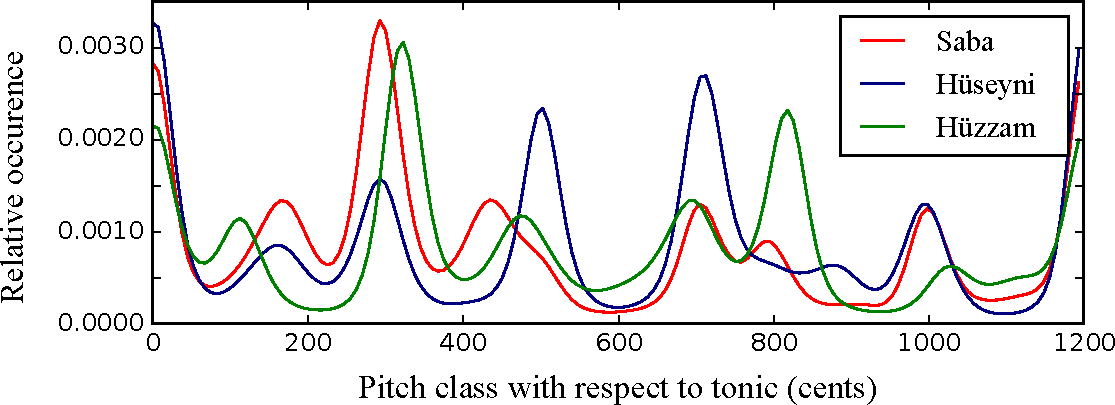
\includegraphics[width=.80\columnwidth]{figures/bozkurt_pcd}
\caption{An example model with single PCD per mode trained for three makams}
\label{fig:bozkurt_training}
\end{figure}

\begin{figure}
\centering
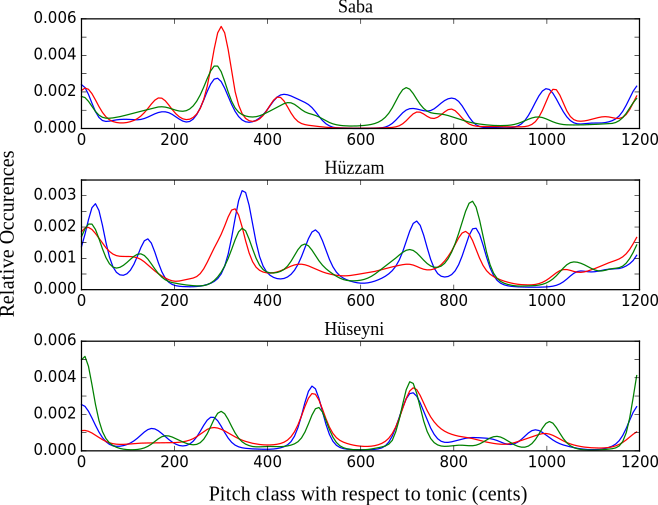
\includegraphics[width=.95\columnwidth]{figures/chordia_pcd}
\caption{An example model with three PCDs per mode trained for three makams}
\label{fig:chordia_training}
\end{figure}

The fundamental difference between the methods proposed in~\cite{bozkurt_makam} and~\cite{chordia} is the training model {\bf (M)} obtained in the training step. The methodology proposed by~\cite{bozkurt_makam} joins all the normalized predominant melodies and compute a single PD or PCD per mode.~\cite{chordia} creates a separate distribution from each annotated excerpt $(a)$. From a machine learning perspective~\cite{bozkurt_makam} represents each mode with a single data point (Figure~\ref{fig:bozkurt_training}), whereas~\cite{chordia} represents them with many (Figure~\ref{fig:chordia_training}) in an $N$-dimensional space, where $N$ is the number of bins in the distributions. From now on, we term the training models using the training step in~\cite{bozkurt_makam} and~\cite{chordia} as ``single distribution per mode'' and ``multi-distributions per mode'', respectively. We denote the obtained model as $M \triangleq \{m_1, m_2, \dots\}$. $m_j \in M$ is a tuple $\langle h_j, \zeta_j\rangle$, where $h_j$ and $\zeta_j$ denotes the trained distribution and the mode label of $m_j$, respectively. The model $M$ consists of the distribution representations for $V$ modes, where $V$ is the number of unique mode labels $\zeta_v, v \in [1:V]$ in the training excerpts.


\section{Nearest Neighbor Selection}\label{sec:distance}
In mode recognition, tonic identification and joint estimation tasks (Section~\ref{sec:mode}-\ref{sec:joint}), the basic step is to find the nearest neighbor(s) of a selected distribution among a set of distributions to be compared against. To find the nearest neighbors we compute a distance or a dissimilarity between the test distribution and each distribution in the comparison set~\cite{distance}. We have currently implemented the distance and the similarity metrics in~\cite{bozkurt_makam, chordia}, namely, City-Block ($L_1$ Norm) distance, Euclidean ($L_2$ Norm) distance, $L_3$ Norm, Bhattacharyya distance, intersection and cross correlation {\bf (P3)}. Note that intersection and cross correlation are similarity metrics, hence we convert them to dissimilarities (i.e. $1 - $similarity) instead. The choice of the distance or dissimilarity measure plays a crucial role in the neighbor selection.

After the distances or the dissimilarities are computed, the compared distributions are ranked and the $k$ {\bf (P4)} nearest neighbors are selected. We then estimate the test sample as the most common label ($\zeta_v$) of the neighbors. In case of a tie between two or more groups, we select label of the group, which accumulates the lowest distance or dissimilarity. Note that if a single-distribution is computed for each mode ({\bf M} as explained in Section~\ref{sec:training}), the $k$ value is always 1, since each mode is only represented by one sample.

Now we proceed to explain the procedure for each task {\bf(T)} in detail.

%The implemented metrics are given below:
%
%\begin{itemize}[noitemsep]
%\item City-Block ($L_1$ Norm) Distance:
%\begin{equation}
%\frac{1}{M}\sum\limits_{m=1}^{M}|h^{(r)}_m - h^{(t)}_m|
%\end{equation}
%
%\item Euclidean ($L_2$ Norm) Distance:
%\begin{equation}
%\sqrt{\sum\limits_{m=1}^{M}\left(h^{(r)}_m - h^{(t)}_m\right)^2}
%\end{equation}
%
%\item $L_3$ Norm:
%\begin{equation}
%\left(\sum\limits_{m=1}^{M}|h^{(r)}_m - h^{(t)}_m|^3\right)^{1/3}
%\end{equation}
%
%\item Bhattacharyya Distance:
%\begin{equation}
%-\log\sum\limits_{m=1}^{M}\sqrt{h^{(r)}_mh^{(t)}_m}
%\end{equation}
%
%%\item Jensen-Shannon Distance:
%%\begin{equation}
%%\sum\limits_{m=1}^{M}XX
%%\end{equation}
%%
%%\item Jeffrey's Divergence:
%%\begin{equation}
%%\sum\limits_{m=1}^{M}XX
%%\end{equation}
%
%\item Inverse of Intersection:
%\begin{equation}
%\left(\frac{1}{M}\sum\limits_{m=1}^{M}min\left(h^{(r)}_m, h^{(t)}_m\right)\right)^{-1}
%\end{equation}
%
%\item Negative of Cross-Correlation:
%\begin{equation}
%1 - \frac{1}{M}\sum\limits_{m=1}^{M}h^{(r)}_m h^{(t)}_m
%\end{equation}
%\end{itemize}
%
%\noindent
%where $h^{(r)}_m$

\section{Mode Recognition}\label{sec:mode}
Given an audio excerpt $(b)$ with an unknown mode, we compute the distribution $h^{\left(b, r^{(b)}\right)}$ by taking the annotated tonic $r^{(b)}$ as the reference (Section~\ref{sec:feature}). Next we compute the distance or the dissimilarity between $h^{\left(b, r^{(b)}\right)}$ and the trained distribution $h_j$ of each $m_j$, $\forall m_j \in M$, where $M$ is the trained model, and obtain the $k$ nearest neighbors to $(b)$. We estimate the mode of $(b)$ as the most common label $\zeta_v$ within the nearest neighbors as explained in Section~\ref{sec:distance}.

\section{Tonic Identification}\label{sec:tonic}

Given an audio excerpt $(b)$ with the annotated mode $\zeta^{(b)}$, we first extract the predominant melody $X^{b}$. Then we compute a distribution $h^{(b, *)}$ by taking an arbitrary frequency $(*)$ as the reference frequency (Section~\ref{sec:feature}). We detect the peaks in the distribution using the method explained in~\cite{smith1987parshl}. The peaks indicate the stable pitches performed in the excerpt. We only consider the peaks, which have a ratio between its height and the maxima of the distribution above a constant threshold {\bf (P5)}. We denote the set of tonic candidates as $R \triangleq \{r_1, \dots, r_W\}$, where $W$ is the number of detected peaks. The cent distance between $r_w$ and $*$ (Equation~\ref{eq:cent_norm}) is given as $r_w^{(*)} = \left(n_w - n_*\right) \times \beta,\,\forall l \in W$, where $\beta$ denotes the bin size {\bf (P1)} of the distribution {\bf (F2)}, and $n_w$ and $n_*$ are the bin indices, in which $l$ and $*$ reside in, i.e. $\lambda_{n_{l}}(l) = \lambda_{n_{*}}(*) = 1$ (Equation~\ref{eqn:histogram}). Assuming each of the peaks $r_w$ as the tonic candidate, we shift the distribution $h^{(b, *)}$ and obtain $h^{(b, r_w)}$ such that the $n$-th bin becomes the $(n + n_* - n_w)$-th for the PDs and the $(n + n_* - n_w \, mod \, K)$-th (where $K$ is the total number of bins) for the PCDs, respectively and the $n_w$-{th} bin represents $0$ cents in the shifted distribution.

From the training model M, we select all the $m_j$'s $\in M$ with the label $\zeta^{(b)}$. Next we compute the distance or the dissimilarity between the each shifted distribution $h^{(b, r_w)}$ and the selected $m_j$. We select the $k$ pairs with the lowest distance or dissimilarity and select the most occurring peak $r_w$ in the neighbors as the estimated tonic (Section~\ref{sec:distance}).

\section{Joint Estimation}\label{sec:joint}
Given an audio excerpt $(b)$ with unknown mode and tonic, we compute the tonic candidates, $R \triangleq \{r_1, \dots, r_W\}$ and the distributions $h^{(b, r_w)}$ assuming each $r_w \in R$ as the tonic candidate as explained in Section~\ref{sec:tonic}. Next we compute the distance or the dissimilarity between each shifted distribution $h^{(b, r_w)}$ and the $m_j$'s in the training model M. We select the $k$ pairs with the lowest distance or dissimilarity and estimate the most occurring $\langle$mode, tonic candidate$\rangle$ pair, i.e.  $\langle \zeta_v, r_w \rangle$ as the mode and the tonic (Section~\ref{sec:distance}).

%For these estimation problems, one of the distinguishing features of a recording is the occurrence frequencies of pitches XXcite, which is called the recording's \textit{pitch distribution} or \textit{PD}. It is computed by extracting the predominant melody of the recording and computing its normalized histogram. We discretize the frequencies, by defining a bin size. We map the frequencies within this range to the same bin. This range should be narrow enough to be informative and wide enough to prevent redundancy, hence it is our first parameter to be tuned.
%
%Even the optimally discretized PDs still have redundancy in them. For our purposes, some frequencies contribute to neither discrimination of modes nor identification of stable pitches. These frequencies appear due to various musical events like vibratos and slides, as well as factors like timbre and dynamics of instruments used, which are out of this work's scope. Following this observation, we consider a more compact and higher level derivative of this feature. \textit{Pitch class distribution} or \textit{PCD} is the octave wrapped version of PD. In other words, unlike PD, PCD exploits the octave information to map the occurrences of different frequencies of the same pitch class to the same value. For example, while PD represents 110 Hz, 220 Hz and 440 Hz as independent frequencies, PCD is informed about the harmonic relationship between these and maps them to the same bin. Hence, PCD provides a more compact representation for distribution of pitches. Clearly, the octave information is lost in this step, but since we are possibly dealing with heterophonic recordings of instruments which don't necessarily have the same spectral ranges, the lost information isn't really informative, but acts as noise for our purposes. Note that if PCD is used as the feature in the tonic identification process, we find the tonic pitch class, the octave is sometimes ambiguous in different cultures, but there are straightforward culture-specific methods~\cite{sercan_tonic,sankalp_tonic}
%
%These two features collectively are referred to as \textit{pitch histograms}. It is possible to smoothen pitch histograms by using methods like kernel density estimation~\cite{chordia} or moving averaging~\cite{bozkurt_tonic} before normalizing them. This process combines the local adjacent peaks and reduces the number of peaks by filtering out the spurious neighbor peaks around the stable pitches. In our implementations, we are using a Gaussian kernel for this procedure. It is possible to improve the algorithms' efficiency with this step, since the number of peaks of a pitch histogram substantially influences the computational cost of processing it, as peaks are treated as the set of tonic candidates. 
%
%As mentioned in Section 1, the tonic information allows us to computationally compare recordings uniformly. The way to do so is to represent the frequencies in the predominant melody with respect to their distance from a reference frequency. If the tonic is known it is treated as the reference point, but during the tonic estimation process, we use a dummy reference frequency since tonic is unknown. The unit that gives us this opportunity is cent. The conversion of a frequency value in Hz units to cents can be done using the following equation.

%Since our goal is to obtain culture-independent tools, we make the bin size parameter variable as mentioned in Section 4. In applications specific to modal music domain, there are many state of the art algorithms based on pitch histograms, such as ...(makam, raga, raag) citeXX. This demonstrates the representative nature of this feature when it comes to recordings of modal music traditions. Moreover, pitch histograms are computationally very convenient. They allow us to represent recordings with a vector of much smaller size compared to sparser alternatives such as the predominant melody or spectrogram of the recording. This shrinkage in data to be processed, impacts the performance of the methods, which would be crucial for real-time applications and big data tasks, such as analyzing entire digital libraries or corpora.

 
%\section{Single Histogram Mode Models}
%Single histogram mode models was proposed as a method specific to OTMM culture, by Gedik \& Bozkurt for tonic identification~\cite{bozkurt_tonic} and makam~\cite{bozkurt_makam} recognition. This approach is based on computing pitch histograms for modeling each mode and using these as the data points for representing the corresponding makams. Then, depending on the problem it uses the distance of the input recording's histogram with makam models in the prediction step. The paper does not report experiments on the joint estimation problem and assumes that one of the two parameters is known beforehand.
%
%First step of building a makam model is to extract the predominant melodies of the recordings that belong to that class. Then, the frequency values in these vectors are converted to cents and joined together to form a long predominant melody vector in cents. The pitch histogram of which is computed and used as the feature to represent the makam. Computationally, this is a very efficient approach, since each makam is represented by a single pitch histogram. The training process of this method consists of these steps and is completed when the pitch histogram representations of all makams are computed.
%
%For makam recognition, the computed makam models are loaded and the pitch distribution of the input recording is computed using the same parameters as in the training phase. Then, the input pitch histogram is compared using a chosen distance formulation. The makam estimate of the method is the one whose pitch histogram has the smallest distance from the input recording's.
%
%For tonic identification, the pitch histogram is computed using a dummy reference frequency and the peaks in this representation are detected. Then, the histogram is compared with the histogram of its known makam by treating each of these peaks as candidate tonics and shifting them to 0 cent frequency. Whichever peak gives the smallest distance is the predicted tonic frequency of the recording.
%
%When we analyzed this approach, we saw some room for improvement and introduced some extensions. As the pitch histogram representation, Bozkurt only uses PD. We included PCD in our implementations, which substantially improved the accuracy of this method in each of the three problems. We added $L_3$ norm to the set of candidate distances.
%
%In order to fully span our framework, we extended this approach to joint estimation problem. In that scenario, the distances are calculated for each peak frequency and mode combination and the pair which has the smallest distance is chosen as the predicted mode and tonic.
%
%\section{Multi-Histogram Representation of Modes}
%The other method we consider is proposed by Chordia \& Şentürk for joint estimation problem~\cite{chordia}. This method was proposed for joint tonic and raag recognition for Hindustani music culture, which we again extend to a general purpose framework for any modal music culture under inspection. 
%
%Unlike histogram mode models approach, this method treats each training sample's pitch histogram as a labeled data point in the feature space. So, the raags are represented with as many points as the available number of recordings in the training dataset. Other than this different perspective of representation, this method is very similar to single-histogram mode model approach~\cite{bozkurt_makam,bozkurt_tonic}. As a demonstration of this representation, Figure 3 shows five three chosen recordings per three makams from our dataset. With this representation, it is possible to capture the nuances within a mode by storing numerous performances that introduce slight variations from it.
%
%The training phase consists of pitch histogram generation of recordings. However, the estimation phase is different due to the multi-point representation. For joint estimation, we consider the \textit{k} many peak and mode pairs that give rise to the smallest distances and the prediction for each is determined by the majority vote among these. In case of a tie, we pick the one with the closest data-point to the input recording's histogram. Hence, we introduce \textit{k} as another adjustable parameter for this method.
%
%For the sake of consistency and completeness, we extend this approach to tonic recognition and mode estimation. Similarly, these predictions are done with the majority vote among the k data-points that give rise to the smallest distance measures. Notice however that, in both cases, it is possible to have these neighbors with different recordings of the same mode, since they are treated equally. Because of this, the number of representations for each mode should be equal, as the mode with more data-points might dominate not because of the similarity but because of its high population. 
%
%Originally, this method is applied to chunks of recordings to the nature of raags. In the original paper that this method was proposed, each recording is sliced into chunks pre-defined length and there are more data-points than the number of recordings in the dataset. In that case, the equal representation is achieved not with the equal number of recordings per mode, but by equal total length of recordings. Another change from the original method was the ability to handle PDs. The original approach is only defined on PCDs, which is expected to outperform the PD counterpart due to the redundancy of the latter. With our implementation and experiments, we quantified the impact of type of pitch histogram on the method's performance. The distance methods applied are the same as the ones for histogram mode models approach. Hence, we are able to compare the performances of these two state of the art algorithms.

\section{Experiments}\label{sec:experiments}
In this section, we provide the results of the experiments we did with the implementations provided in MORTY. We did exhaustive experiments using our dataset to demonstrate some properties of these methods, find the best parameter sets for OTMM and to provide some heuristics for future users. For the sake of reproducability all of the scripts, computed features, experiments and results are shared online\footnote{\url{https://github.com/sertansenturk/dlfm_makam_recognition}}.

\section{Test Dataset}\label{sec:dataset}

In~\cite{bozkurt_makam}, the makam recognition methodology was evaluated on 172 solo audio recordings in 9 makams. To the best of our knowledge, this dataset represents the biggest number of recordings that has been used to evaluate makam recognition task, so far. As explained by the authors~\cite{bozkurt_makam}, these recordings were selected from the performances of ``indisputable masters,'' and therefore they are musically representative of the covered makams. Nevertheless the results are not reproducible as the datasets are not provided by the authors. 

The tonic identification methodology proposed by~\cite{bozkurt_makam} was evaluated using 150 synthesized MIDI files plus 118 solo recordings. As explained in the above paragraph, the data is not available. To the best of our knowledge there exists only two open tonic identification datasets for OTMM, both of which are compiled under the CompMusic project.\footnote{http://compmusic.upf.edu/} The first one is provided in~\cite{senturk2013karar_ismir} and it consists of 257 audio recordings. The second and the bigger test dataset is provided in~\cite{sercan_tonic}, consisting of 1093 recordings\footnote{The datasets are hosted in \url{https://github.com/MTG/turkish_makam_tonic_dataset/releases/}}. The recordings in both of the datasets are identified using MusicBrainz MBIDs\footnote{\url{https://musicbrainz.org/doc/MusicBrainz_Identifier}}. The authors use a predominant me\-lody extraction method proposed by~\cite{salamon2012melody} optimized for OTMM~\cite{atli2014makamFeature_atmm}, which they have opened later\footnote{https://github.com/sertansenturk/predominantmelodymakam}. Nevertheless, the predominant melodies extracted from the audio recordings are not provided in either dataset.
 
Considering the lack of open test datasets for makam re\-cognition and the drawbacks of the available tonic identification datasets, we have gathered a test dataset of audio recordings with annotated makam and tonic, called the \emph{Ottoman-Turkish makam recognition dataset}.\footnote{\url{https://github.com/MTG/ottoman_turkish_makam_recognition_dataset}} The data\-set covers 20 commonly performed makams\footnote{i.e. Acema\c{s}iran, Acemk\"{u}rdi, Bestenigar, Beyati, Hicaz, Hicazkar, H\"{u}seyni, H\"{u}zzam, Karc{\i}\u{g}ar, K\"{u}rdilihicazkar, Mahur, Muhayyer, Neva, Nihavent, Rast, Saba, Segah, Sultan{\i}yegah, Suzinak and U\c{s}\c{s}ak} and it is composed of 1000 audio recordings (i.e. 50 recordings per makam) in total. To the best of our knowledge, our dataset is the largest and the most comprehensive dataset for the evaluation of automatic makam re\-cognition. Moreover, it is comparable to the dataset provided in~\cite{atli2014makamFeature_atmm} for the evaluation of tonic identification methodologies.

Similar to~\cite{senturk2013karar_ismir} and~\cite{sercan_tonic}, the recordings in the dataset are labeled with MusicBrainz MBIDs. The tonic frequency of each recording is annotated manually using the procedure explained in~\cite{senturk2013karar_ismir} and the annotations are cross checked by at least two annotators. For reproducibility reasons, we also include the predominant melodies extracted from the audio recordings. We use the open implementation of the predominant melody extraction methodology in~\cite{atli2014makamFeature_atmm}. We additionally filter the predominant melody to get rid of the spurious estimations and correct the octave errors as explained in~\cite{bozkurt_tonic}. To the best of our knowledge this procedure~\cite{atli2014makamFeature_atmm} currently outputs the most reliable predominant melody estimations for OTMM. 

Similar to~\cite{bozkurt_makam}, the dataset is intended to be musically representative of OTMM. To achieve this, we selected the recordings of acknowledged musicians from the CompMusic makam corpus, which is currently the most representative music corpus of OTMM aimed at computational research~\cite{compmusic_corpus}. The dataset covers contemporary and historical, monophonic and heterophonic recordings, as well as live and studio recordings. Some of the recordings have non-musical sections, such as clapping at the end of live recordings, announcements in radio recordings or scratch and hissing sounds throughout the historical recordings. Pie chard of the instrument vocal etc.XX This diversity gives us the opportunity to test the methods in a much more challenging environment, which hasn't been completely addressed in the previous research~\cite{bozkurt_makam}. Following our assumption in the problem definition, each recording belongs to a single makamXXrephrase.

\section{Experimental Setup}\label{sec:experiment_setup}
In the experiments we use stratified 10-fold cross validation. Table~\ref{tab:performanceKDoc} gives a combination of the parameters used in the experimental setup. We use grid search, to find the optimal parameters for OTMM (Section~\ref{sec:methodology}). {\bf (F1)} is selected as the state of the art in predominant melody extraction for OTMM. The parameter combinations where the bin size $\beta$ is greater than or equal to $3$ times the kernel width $\sigma$ are omitted. We also conduct experiments where the distribution smoothing is skipped. When the training model consists of a ``single'' distribution per mode, the number of neighbors $k$ is always taken as 1 as each label is represented by a single data point. The minimum peak ratio {\bf (P5)} is only used in tonic identification and its optimal value is found separately as will be explained in Section~\ref{sec:results}.

\begin{table*}
\caption{The summary of the parameters tried in the experiments}
\begin{center}
\begin{adjustbox}{max width=0.95\textwidth}
 \begin{tabular}{l l p{0.35\textwidth} p{0.45\textwidth}}
 \noalign{\hrule height 1.2pt}
& Name & Values & Comment\\
\hline
{\bf T} & task & mode, tonic, joint & \\
{\bf F1} & predominant melody, $X$ & \hspace{1sp}\cite{atli2014makamFeature_atmm} & extraction method specialized for OTMM\\
{\bf F2} & distribution, $h$ & PD, PCD\\
{\bf M} & type of the training model, $M$ & single, multi & number of distribution per mode used in~\cite{chordia, bozkurt_makam} \\
{\bf P1} & bin size, $\beta$ & $7.5, 15, 25, 50, 100$ cents \\
{\bf P2} & kernel width, $\sigma$ & ``no smoothing \& $7.5, 15, 25, 50, 100$ cents'' & Combinations with $\beta \geq 3\sigma$ are omitted. \\
{\bf P3} & distance or dissimilarity & L$_1$, L$_2$, L$_3$, Bhattacharyya, $1 -$intersection,  $1 -$cross\_correlation & $1 -$intersection and $1 -$cross\_correlation are dissimilarities computed from the namesake similarity measures\\
{\bf P4} & number of nearest neighbors, $k$ & $\{1, 3, 5, 10, 15\}$ & for the ``single'' distribution per mode training model,  the value is fixed to $1$\\
{\bf P5} & minimum peak ratio & $[0, 1]$ & with a step of $0.5$, only for tonic identification and joint estimation\\
 \end{tabular}
 \end{adjustbox}
\end{center}
 \label{tab:performanceKDoc}
\end{table*}

For mode recognition, we mark the classification is $True$ if the estimated mode and the annotated mode for a recording are the same. The tonic octave in the orchestral performances of OTMM is ambiguous as each instrument plays the melody in their own register. Therefore, we aim identify the tonic pitch class. We calculate the octave wrapped cent distance between the estimated and the annotated tonic, i.e. $min\left(\bigl(|e^{(r)}|\,\bmod\,1200\bigr), 1200-\bigl(|e^{(r)}|\,\bmod\,1200\bigl)\right)$, where \\$\bmod$ is the modulo operation. Remember that $e^{(r)}$ is the normalization of the estimated tonic frequency $e$, with respect to the annotated tonic frequency $r$ (Equation~\ref{eqn:histogram}). If the cent distance is less than $25$, we consider the tonic identification as correct. In the case of joint estimation, we require both tonic and mode estimates to be correct. 

For each fold we compute the accuracy, which is the number of correct estimations divided by the total number of testing data. In Section~\ref{sec:results}, we
report the average accuracies of the folds for each parameter combination. For all results below, the term ``significant'' has the following means that the claim is statistically significant at the $p = 0.01$ level as determined by a multiple comparison test using the Tukey-Kramer statistic.

We additionally compare the tonic identification results obtained in the tonic identification and joint estimation tasks with the results obtained from the current state of the art in OTMM~\cite{sercan_tonic}. The method is based on detecting the last stable pitch of the recording, which is typically the tonic.\footnote{The open implementation is available at \url{https://github.com/hsercanatli/tonicidentifier_makam}}.

\section{Results}\label{sec:results}
Minimum peak ratio experiment XX

Table \ref{tab:best_results} shows the best results obtained after grid search. For mode recognition, multiple distribution per mode model yields an accuracy of 70.6\% with the best parameter set and the single distribution per mode method yileds a slightly higher accuracy of 71.4\%. For tonic identification multiple distribution per mode performs with above 94\% accuracy in 49 sets and above 90\% accuracy in 180 parameter sets out of 540 experiments, where the highest accuracy obtained is 94.9\%. Hence, the method is robust to a variety of parameter selections for tonic identification. Single distribution per mode model performs on par with the multi-model approach and yields 94.5\% accuracy with the best parameter set. The method proposed by ~\cite{sercan_tonic} performs with 79.9\% accuracy in tonic identification on our dataset. For joint estimation the distribution per mode model performed with 63.2\% accuracy in the optimal configuration while multi-distribution yielded 62.1\%.

In both methods and all three tasks, the distance method of all best parameter sets turned out to be Bhattacharyya distance and the histogram type to be PCD.

\begin{table}
\label{tab:best_results}
\caption{Best parameter sets for each task and method.}
 \begin{center}
%\begin{tabular}{ |l|l|l|l|l|l| }
\begin{tabular}{ l l c c c c }
\hline
\textbf{Task} & \textbf{Method} & \textbf{sf} & \textbf{ss} & \textbf{k} & \textbf{Accuracy}\\ \hline
\multirow{5}{*}{Tonic} & \multirow{3}{*}{Multi} & 15 & 15 & 3 or 5 &\multirow{3}{*}{\textbf{94.9\%}}\\
 & & 15 & 7.5 & 5 &\\
  & & 0 & 7.5 & 3 &\\
 \cline{2-6}
 & Single & 20 & 7.5 & - & 94.5\% \\ \hline
\multirow{2}{*}{Mode} & Multi & 20 & 25 & 5 & 70.6\% \\
\cline{2-6}
& Single & 15 & 7.5 & - & \textbf{71.4\%}\\ \hline
\multirow{2}{*}{Joint} & Multi & 20 & 15 & 5 & 62.1\%\\
\cline{2-6}
& Single & 15 & 7.5 & - & \textbf{63.2\%}\\ \hline
\end{tabular}
\end{center}
\end{table}
These experiments revealed that certain parameter selections significantly improve or diminish the methods' performances. These observations are listed below as heuristics for future users.
\begin{itemize}[noitemsep]
\item Single-histogram mode models approach perform slightly better than multi-histogram models. The difference is insignificant.
\item PCD significantly outperforms PD.
\item Bhattacharyya, intersection and city-block distance significantly outperform cross-correlation, $L_3$ and Euclidean.
\item Smaller bin size yield better results, however there is no significant between 7.5, 15 and 25 cent bin sizes. Note that these bin sizes significantly outperform 50 and 100 cent bin sizes.
\item Increasing smoothing above 7.5 cents improves the accuracy of the models, but this change is not significant.XX
\item In the case of multi-distribution per mode model, the value of $k$ does not make a significant impact, however a $k$ value of 5 performs better.XX
\end{itemize}

Confusion matrix XX

\section{Experiments on Hindustani and Carnatic Music}
\label{sec:hindustani_carnatic}

Recently, MORTY had been used as a benchmark for raga/raag recognition of audio recordings of Hindustani and Carnatic music in comparison with two novel methods~\cite{gulati_network, hindustani_carnatic_experiments_anon}. In the experiments we use the optimal parameters reported in~\cite{chordia}: We compute pitch class distributions with a bin size of $\beta=10$ cents. The kernel width $\sigma$ reported in~\cite{chordia} is in Hz scale, which is would mean variable smoothing across octave. We empirically found $\sigma = 15$ cents as a reasonable value. We train multiple pitch class distributions per mode as described in~\cite{chordia}. In testing we use Bhattacharyya distance and select the nearest neighbor ($k = 1$). Note that there already exists a method for tonic identification for these music traditions~\cite{sankalp_tonic}, which is reported to provide near perfect results. We use this method for the automatic tonic identification instead of the methodology explained in Section~\ref{sec:training}. Below we explain the results briefly. Please refer to the respective papers~\cite{gulati_network, hindustani_carnatic_experiments_anon} for further details.

In~\cite{gulati_network} a method based on melodic contours is proposed for mode recognition. The method is compared against the methods proposed in~\cite{chordia} (our method) and~\cite{koduri2014intonation} on two datasets consisting Carnatic music recordings in 10 ragas and 40 ragas, respectively. The best accuracies obtained for the 10 raga dataset are $91.7\%$, $89.5\%$ and $70.01\%$ using the proposed method, MORTY and~\cite{koduri2014intonation}. Both the proposed methodology and MORTY obtained comparable results and they outperformed~\cite{koduri2014intonation}. In the 40 raga dataset our method ($74.1\%$ accuracy) outperformed the both methods the proposed method ($69.6\%$ accuracy) and ~\cite{koduri2014intonation} ($51.4\%$ accuracy).

Later the same authors have proposed another feature for raga recognition~\cite{hindustani_carnatic_experiments_anon}, which they term as ``time-delayed melody surface.'' The training and testing scheme is the same with the procedure explained in~\cite{chordia}. In the experiments The proposed feature was compared against pitch class distributions on a dataset of Hindustani recordings and the same dataset used in~\cite{gulati_network} with a different experimental setup. In both datasets the proposed feature ($97.7\%$ accuracy on Hindustani and $86.7\%$ accuracy on Carnatic dataset) has outperforms PCDs ($91.7\%$ accuracy on Hindustani and $73.1\%$ accuracy on Carnatic dataset).

% \section{Multi-Layer Perceptron Network}\label{sec:neuralnet}
% Multi-layer perceptron network (MLP) or fully connected neural network~\cite{neural_textbook} is one of the most commonly used general purpose neural network architectures in the literature. As a primer work on applying neural networks on culture-independent modal music information retrieval, we decided to use this architecture, due to its established theory and convenience for theoretical computations. 
% 
% In different contexts, MLPs are shown to perform substantially better as the amount of training data is increased~\cite{ciresan}. Having curated the largest OTMM recording dataset in the literature, we had already overcome a challenging prerequisite for using neural networks for these task, considering the lack of available public datasets for the domain.
% 
% As described in more detail in the following section, this dataset is composed of 1000 recordings, distributed as 50 recording for each of 20 most common makams in CompMusic corpus~\cite{compmusic_corpus}. Hence, we define our problem as 20-class mode recognition with a training dataset of 1000 samples.
% 
% Since the complexity of the network and hence the data required to train it is proportional to the number of nodes in the network~\cite{vc-dimension}~\cite{bartlett}, we decided to use PCD as the network's input feature, instead of PD. In addition to its ability to represent the recordings more compactly, the fixed size of PCD make it a much more convenient choice than the variable length and variable range alternative PD. With the same motivation, we decided to use a MLP with a relatively small size, with no hidden layers, input layer of size equal to the size of PCD and an output of size equal to number of classes. The output of each output neuron would be treated as the confidence of the network of the input belonging to the corresponding class. The highest confidence, in other words the index of maximum value from the output layer, is treated as the network's estimate of mode.
% 
% One of the most challenging steps of theoretical studies on neural networks, is representing the complexity of the network, which can be quantified by the size of the network's hypothesis set, \textit{H}. The hypothesis set is a function space which spans the possible functions the neural network might converge to, through training. Since it is very hard to estimate this parameter, it is common to work with growth functions, denoted by \textit{$m_H(N)$}. It refers to the growth of the hypothesis set with the increase of number of samples, denoted here with \textit{N}. More concretely, \textit{$m_H(N)$} denotes the most number of dichotomies that \textit{H} implements over all possible training sets of size \textit{N}. One way to work with this value is to use VC-dimension~\cite{vc-dimension}, denoted by $d_{VC}$, as an upper bound on it. As a heuristic, $d_{VC}$ is approximated as the number of parameters~\cite{bartlett} for MLP. We use this approach and the following theorem~\cite{lower_bound} to obtain a lower bound on the required number of samples to be able to train the network we specified fully. 
% 
% \textbf{Theorem~\cite{lower_bound}:} Let \textit{L} be a learning algorithm that uses \textit{H} consistently. Then, given $0 < \epsilon < \frac{1}{8}$ and $0 < \delta < \frac{1}{100}$ and less than \textit{N} random examples, there is some probability distribution that for which \textit{L} will not produce a function $h \in H$, with $error(h) \leq \epsilon$ with probability $1 - \delta$, where:
% \begin{equation}
% N = \frac{d_{VC}(H) - 1}{32\epsilon}
% \end{equation}
% This theorem provides us a lower bound on the number of training samples to ensure that the learning algorithm is trained enough to be able to converge to all functions in its hypothesis set with error less than $\epsilon$ with probability $1-\delta$. When this lower bound for our non-complex network is computed, it shows that even the largest dataset in the literature is far from being enough to ensure this condition. 
% 
% As an example, we consider using 160 dimensional and 80 dimensional PCDs, which correspond to 7.5 cents and 15 cents bin sizes and are typical choices for mode and tonic estimation tasks~\cite{chordia,bozkurt_makam,bozkurt_tonic}. We chose the error margin as $\epsilon=0.1$ and calculated the lower bounds of training set sizes as 9100 and 2550, respectively. Since we only have 1000 recordings available, we don't expect our neural network implementation to be a reliable choice for these tasks, with this configuration. 
% 
% To tackle this problem, we considered using principal component analysis (PCA)~\cite{pca} for dimension reduction, which would diminish the size of the network while preserving the variance among training samples. However, our experiments on our dataset yielded unsatisfactory results. 

\section{Discussion}\label{sec:discussion}

The drawback of the pitch class distribution method is that it does not consider the temporal characteristics. When we inspected the results obtained from the experiments in~\ref{sec:experiments}, we observed that the confusions are mainly between makams, which either have very similar intervals in their scale. Similarly in~\cite{gulati_network}, the proposed method was better in classifying phrase-based ragas, while our method was better at classifying scale based ones. The mode recognition using the feature proposed in ~\cite{hindustani_carnatic_experiments_anon} is able to capture both of these properties better with a slight increase in computational complexity.

Nevertheless,~\cite{sercan_tonic} yields better results in tonic identification when the makam information is not available.

Therefore, our dataset can be used complementary with the earlier tonic datasets~\cite{senturk2013karar_ismir, atli2014makamFeature_atmm}. Our method outperforms~\cite{sercan_tonic}, if the makam of the recording is known. 

In the light of these information and our empirical observations, we suggest using single-histogram models approach with Bhattacharyya distance, PCD, smoothing factor of 20 cents and bin size of 7.5 cents for a system that performs well in all of the three tasks. 


\section{Conclusion}\label{sec:conclusion}

This primary research can be used as a starting point for future works that aim to use neural networks for modal music information retrieval tasks. 

Out of the listed methods that make use of pitch histograms, we decided to focus on single histogram mode models~\cite{bozkurt_makam,bozkurt_tonic} and multi-histogram mode models~\cite{chordia} approaches because the first is the state of the art for mode and tonic recognition tasks in OTMM culture and the latter is for joint recognition for Hindustani, while being on par with the state-of-the-art~\cite{gulati_network} for mode recognition in Carnatic tradition. In addition to these existing methods, we implemented a neural network model for culture-independent multi-mode recognition. The recent vast improvements in neural network methods and the availability of data due to our dataset makes this method a promising candidate for future research on this problem. 



\bibliographystyle{abbrv}
\bibliography{sigproc}  % sigproc.bib is the name of the Bibliography in this case


\end{document}
